\documentclass[12pt]{article}
\usepackage{graphicx}
\usepackage{float} 
\usepackage{hyperref}
\usepackage{amsmath}

\begin{document}
	\begin{center}
		\LARGE{Elastostatic calibration for cylindrical robot}
	\end{center}
	\section{Model}
	\begin{itemize}
		\item Since there are rigid links and flexible joints there are 3 parameters which should be identified \\
		Model scheme:
		\begin{figure}[H]
			\centering
			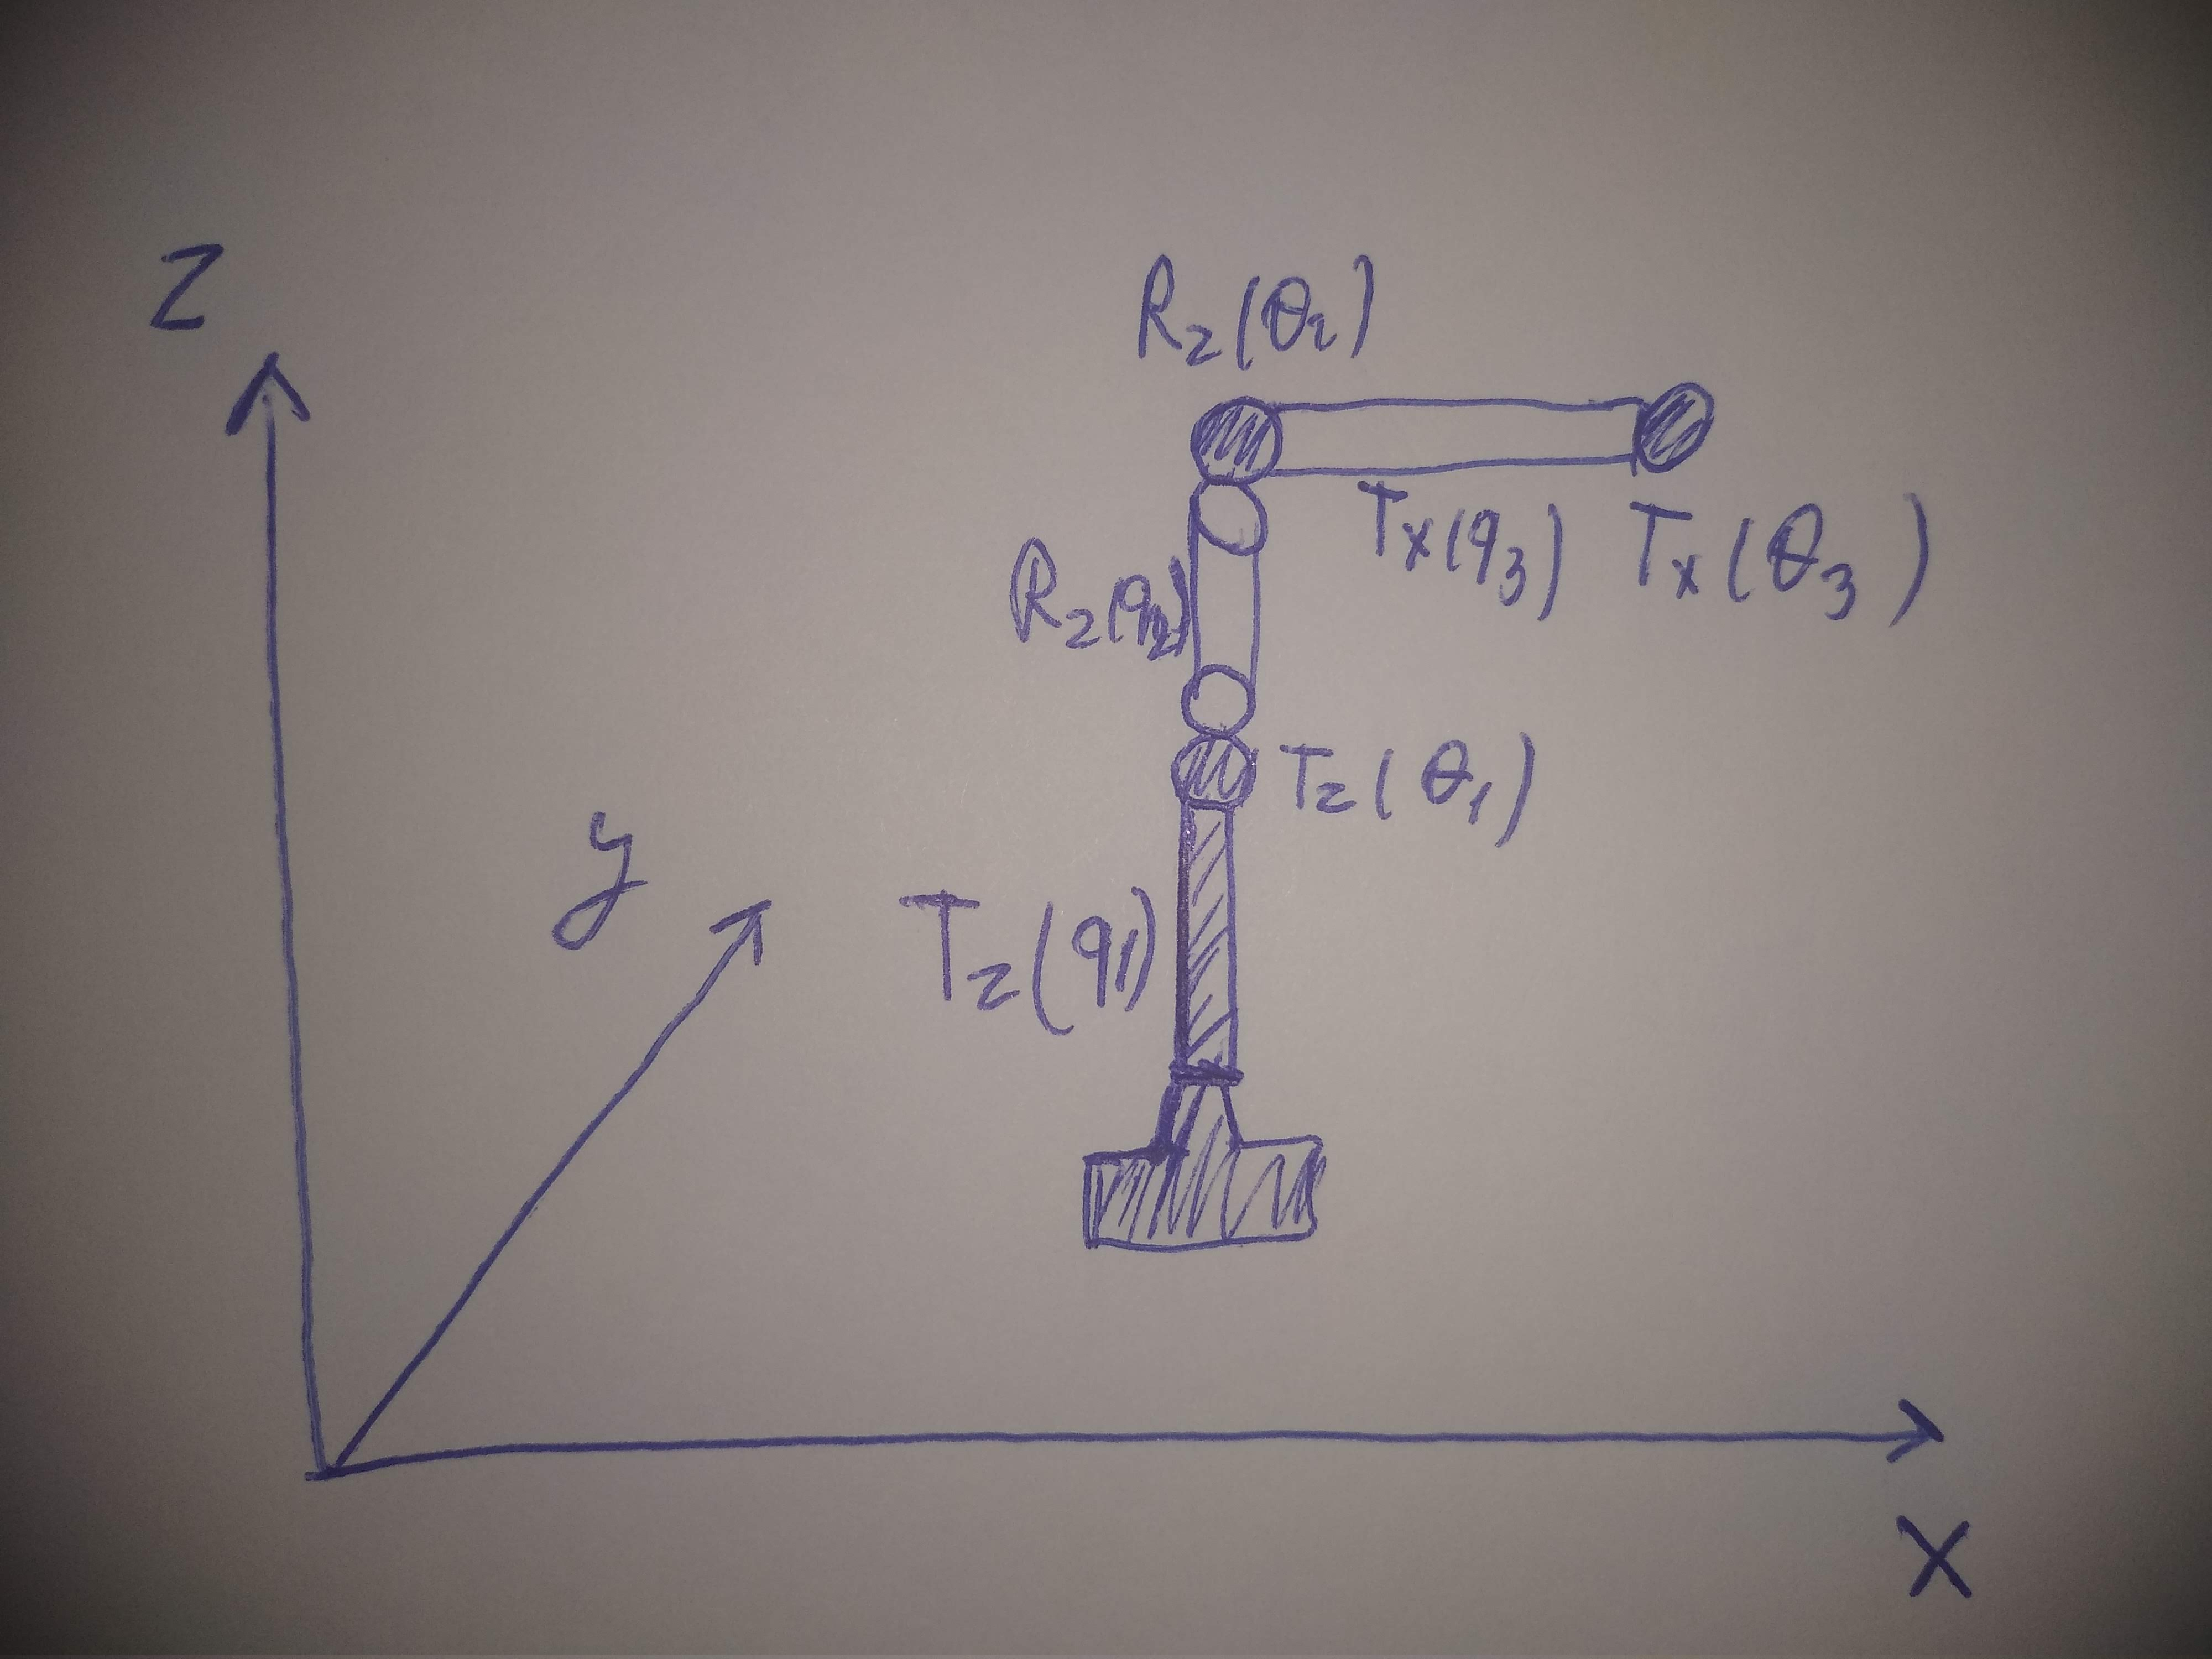
\includegraphics[scale=0.07]{scheme.jpg}
			\caption{Model scheme}
		\end{figure}
	
		\item Direct kinematics for this robot can be written as follows: \\
		\begin{math}
		T = T_{z}(q_1)T_{z}(\theta _{1})R_{z}(q_2)Rz(\theta _2)T_x(q_3)T_x(\theta _3))
		\end{math}
		
		\item Inverse kinematics:
		\begin{itemize}
			\item $q_1 = z$
			\item $q_2 = \arctan2(y, x)$
			\item $q_3 = \sqrt{x^2 + y ^2} $
		\end{itemize}
	
	\end{itemize}

	\section{Calibration process}
	\begin{enumerate}
		\item Create 30 random configuration. Configuration include 3 joints positions and applied range.
		\item Numerically compute jacobians with respect to joints deflections for each configurations.
		\item Compute matrix A where each row has a following form: \\
		$$
			A_i = 
			\begin{bmatrix}
				J_{1i}J_{1i}^T W_i & J_{2i}J_{2i}^T W_i & J_{3i}J_{3i}^T W_i \\
			\end{bmatrix}
		$$
		where $J_1i, J_2i, J_3i$ - Jacobians over 1st, 2nd and 3rd joints deflections on $i^{th}$ configurations, $W_i$ - range applied on $i^{th}$ configuration
		\item Compute real end-effector deflection on each configuration. k - vector real joints parameters (inverse of joint stiffness) given in problem statement, in reality measured by laser tracker
		$$ \Delta t_i = A_i * k $$
		\item Compute joint parameters by formula: 
		$$
			k_{est} = (\sum_{i = 1}^{m}A_i^T A_i)^{-1}  \sum_{i = 1}^{m} A_i \Delta t_i
		$$
		
	\end{enumerate}

	\section{Error correction}
	\begin{enumerate}
		\item Set sequence of points that end-effector should pass and randomly set a load
		\item For each point compute inverse kinematics
		\item Compute deflection in this point based on estimated parameters
		\item Plug to joints position controller inverse kinematics for point which coordinates equal to difference between desired coordinates and deflection.
	\end{enumerate}

	\section{Results analysis}
	\subsection{Without noise in deflection measurement}
	\begin{itemize}
		\item As a result of calibration joints stiffness computed precisely since there is no error in deflection measurement. 
		\item Comparison of desired trajectory and obtained by calibrated and non-calibrated robot (here we can see that desired trajectory ideally coincident with one obtained by calibrated robot)
		\begin{figure}[H]
			\centering
			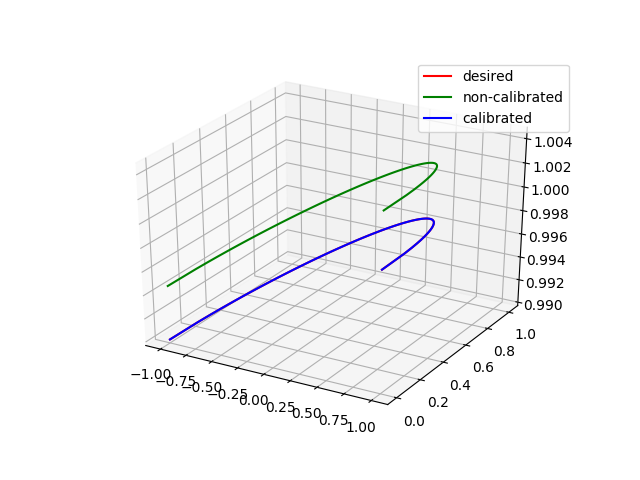
\includegraphics[scale=0.6]{no_noise.png}
			\caption{Trajectories plot}
		\end{figure}
		\item Mean error for non-calibrated robot on x, y and z equal to 4.21, 14.18, 0.66 mm correspondingly.
		
		\item For calibrated robot errors on all direction equal to zero
	\end{itemize}

	\subsection{With noise in deflection measurement}
	\begin{itemize}
		\item In reality the laser tracker used for deflection measurement has some noises
		\item There was also analyzed the calibration result with different noise of laser tracker. Noise treated as normally distributed value with 0 mean
		\item Calibration process remains the same only difference is that we add noise to $\Delta t_i$
		\item If noise variance equal to 0.01mm:
		\begin{figure}[H]
			\centering
			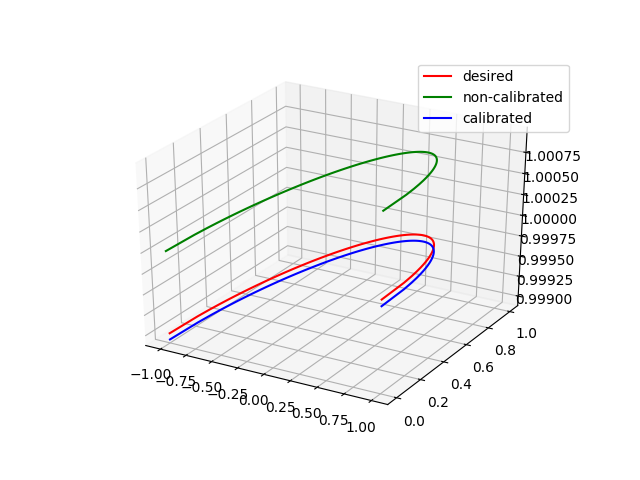
\includegraphics[scale=0.6]{01noise.png}
			\caption{Trajectories plot with 0.01 noise variance}
		\end{figure}
		\item If noise variance equal to 0.05mm:
		\begin{figure}[H]
			\centering
			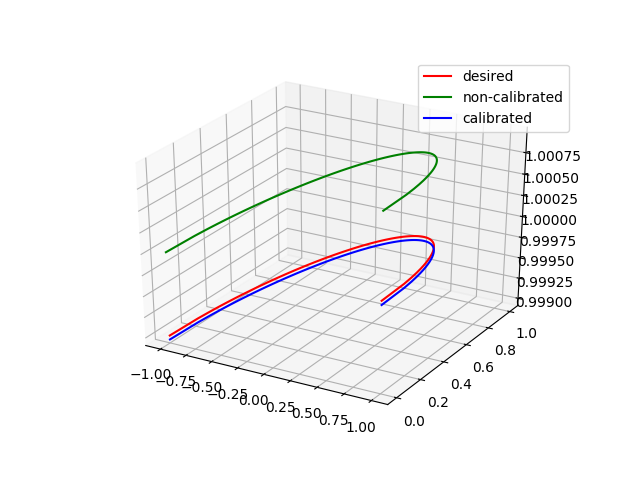
\includegraphics[scale=0.6]{05noise.png}
			\caption{Trajectories plot with 0.05 noise variance}
		\end{figure}
		\item If noise variance equal to 0.1mm:
		\begin{figure}[H]
			\centering
			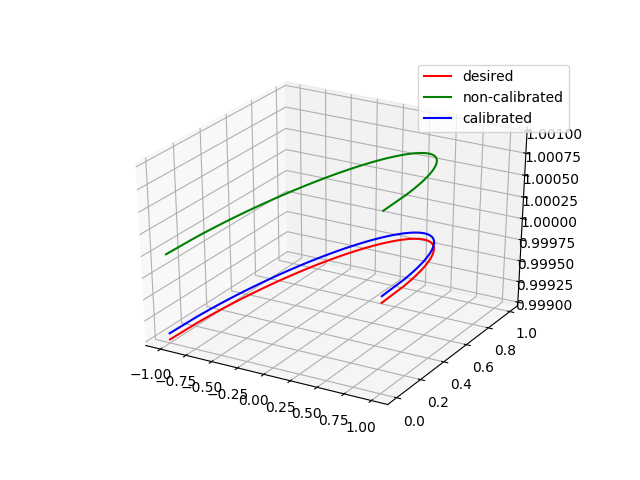
\includegraphics[scale=0.6]{1noise.png}
			\caption{Trajectories plot with 0.1 noise variance}
		\end{figure}
		\item If noise variance equal to 0.5mm:
		\begin{figure}[H]
			\centering
			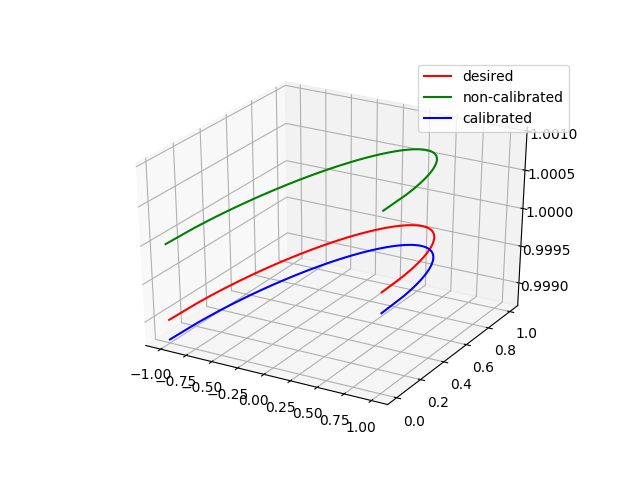
\includegraphics[scale=0.6]{10noise.png}
			\caption{Trajectories plot with 0.5 noise variance}
		\end{figure}
	\end{itemize}

	Table with errors dependent on noise (errors taken with precision up to 6 digits after point, comparison was done with range [1000, 1000, 1000, 1000, 1000, 1000]): \\
	\begin{tabular}{|c| |c| |c| |c|}
		\hline
		Noise variance, m & Mean x error, m  & Mean y error, m & Mean z error, m \\
		\hline
		$10^{-5}$ &  0.000012 & 0.000033 & 0.000077\\
		\hline
		$5 * 10^{-5}$ & 0.000047 & 0.000032 & 0.000193 \\
		\hline
		$10^{-4}$ & 0.000038 & 0.000040 & 0.000308 \\
		\hline
		$5 * 10^{-4}$ & 0.000662 & 0.000819 & 0.000266 \\
		\hline
	\end{tabular}

	\section{Github link:} 
	\href{https://github.com/jenamax/Robotics_Systems/tree/master/Homework2}{\underline{link}}
\end{document}